% ALIGN-PARETO project report.
% Build: pdflatex main && pdflatex main   (run twice so citation numbers resolve; no BibTeX needed)
% or upload this folder to Overleaf. Figures are in figures/, copied from results/.
% References are written in the thebibliography block at the end of this file, numbered in order of first citation.
\documentclass[11pt,a4paper]{article}

\usepackage[T1]{fontenc}
\usepackage[utf8]{inputenc}
\usepackage{lmodern}
\usepackage[margin=2.5cm]{geometry}
\usepackage{amsmath,amssymb}
\usepackage{graphicx}
\usepackage{booktabs}
\usepackage{tabularx}
\usepackage{array}
\usepackage{multirow}
\usepackage{xcolor}
\usepackage[font=small,labelfont=bf]{caption}
\usepackage{enumitem}
\usepackage[colorlinks=true,linkcolor=blue!50!black,citecolor=blue!50!black,urlcolor=blue!50!black]{hyperref}

% Wikipedia-style citations: superscript [1], [2, 3] in the text; numbered list at the end
\makeatletter
\renewcommand{\@cite}[2]{\textsuperscript{[#1\if@tempswa, #2\fi]}}
\makeatother

\setlist{itemsep=2pt,topsep=4pt}
\newcolumntype{L}{>{\raggedright\arraybackslash}X}
\newcommand{\q}[1]{\texttt{#1}}          % quadrant codes, e.g. \q{1\_0}
\newcommand{\lam}{\lambda}

\title{\textbf{ALIGN-PARETO}\\[4pt]
\large Measuring and Reducing the Alignment Tax on Creativity\\ with a Prompt-Adaptive Alignment Strength}
% TODO: replace with the authors' names and the course details.
\author{\small\textit{Author names, course and institution to be added}}
\date{November 2026}

\begin{document}
\maketitle

\begin{abstract}
Safety alignment makes language models safer, but it is widely reported to make their outputs blander and more alike, a cost known as the \emph{alignment tax}. We study this tax for creativity on a small open model and ask whether choosing the alignment strength per prompt can keep safety while losing less creativity. We build an unaligned chat model by supervised fine-tuning Qwen3-0.6B-Base on human-written replies, and define an alignment dial $\lam$ that linearly interpolates its weights with those of Qwen's safety-aligned Qwen3-0.6B. On 400 evaluation prompts, with 5 sampled replies per prompt and every reply judged by Qwen3Guard-Gen-4B, moving from $\lam=0$ to $\lam=1$ raises safety (one minus the harmful-response rate on harmful prompts) from 0.276 to 0.406 and lowers semantic diversity on creative, safe prompts by 31\% (0.313 to 0.215). Every value of $\lam$ is Pareto-optimal, and the loss comes from more homogeneous answers rather than from more refusals. A controller that picks $\lam$ per prompt from a lightweight prompt classifier, calibrated on validation prompts, reaches on held-out test prompts a creativity of 0.280 versus 0.216 for the aligned model (+0.064, 95\% CI [+0.032, +0.097]) at a safety of 0.396 versus 0.402 ($-$0.006, 95\% CI [$-$0.019, 0.000]). Most of the remaining gap to an oracle with true prompt labels is due to the classifier mistaking creative requests for harmful ones. The safety judge's labels have not yet been validated against human labels; we state this as the main open limitation.
\end{abstract}

\section{Introduction}

Aligning a language model for safety, through supervised fine-tuning on curated replies and preference optimisation, changes more than its willingness to help with harmful requests. Recent work reports that aligned models lose capabilities that the pretrained model had\cite{lin2024mitigating}, that their sampled answers collapse onto few distinct meanings\cite{liu2026homogenization}, and that alignment shifts the values a model expresses\cite{chen2026value}. We call these costs the \emph{alignment tax}.

This project measures the tax on one property, \emph{creativity}, understood as the variety of a model's answers to an open-ended request, and asks a practical question: if a single alignment strength forces a trade-off between safety and creativity, can a strength chosen \emph{per prompt} do better? Most prompts are either harmless creative requests, where alignment brings little benefit, or harmful requests, where it is needed. A system that can tell them apart could apply alignment where it matters and keep creativity elsewhere.

\paragraph{Contributions.}
\begin{enumerate}
  \item A controllable alignment dial: linear weight interpolation between an unaligned supervised fine-tuned (SFT) model and an existing aligned model that share the same pretrained base (Section~\ref{sec:m3-method}).
  \item A measured safety--creativity trade-off over five dial settings on 400 prompts and 10{,}000 judged replies, with a length-matched robustness check (Section~\ref{sec:m3-results}).
  \item A prompt-adaptive controller that selects the dial setting from a prompt classifier, calibrated on validation data and evaluated once on held-out test data with paired bootstrap intervals (Sections~\ref{sec:m4-method}--\ref{sec:m4-results}).
\end{enumerate}

\section{Related work}

\paragraph{Alignment tax.} Lin et al.\cite{lin2024mitigating} show that RLHF reduces abilities acquired in pretraining and that averaging the weights of the model before and after alignment gives a better trade-off between reward and retained ability than most other mitigation methods. Our dial applies the same weight-averaging idea between an unaligned and an aligned model. Liu\cite{liu2026homogenization} report \emph{response homogenisation}: aligned models often place all of several sampled answers in one semantic cluster, while the base model does not. We measure the same effect with semantic diversity and cluster counts. Chen and Shen\cite{chen2026value} measure how alignment trades off values against each other; our work restricts attention to the safety--creativity pair.

\paragraph{Weight interpolation.} Interpolating between fine-tuned models that share a pretrained initialisation is known to give coherent intermediate models, as in model soups\cite{wortsman2022soups} and robust fine-tuning by weight-space ensembling\cite{wortsman2022wiseft}. This property is what makes a continuous alignment dial possible without retraining.

\paragraph{Safety moderation.} We use Qwen3Guard\cite{qwen3guard} to judge replies; the prompt data for safety comes from WildGuardMix\cite{han2024wildguard}, which was built for training such moderation models.

\section{Overview}
\label{sec:overview}

The project has four milestones that feed into each other (Figure~\ref{fig:flow}). M1 trains a prompt classifier and provides the evaluation prompts. M2 builds the unaligned end of the dial. M3 sweeps the dial and measures the trade-off. M4 uses the M1 classifier and the M3 results to choose the dial setting per prompt. M2 and M3 ran on a single NVIDIA T4 GPU on Kaggle; M1 and M4 run on a CPU.

\begin{figure}[t]
  \centering
  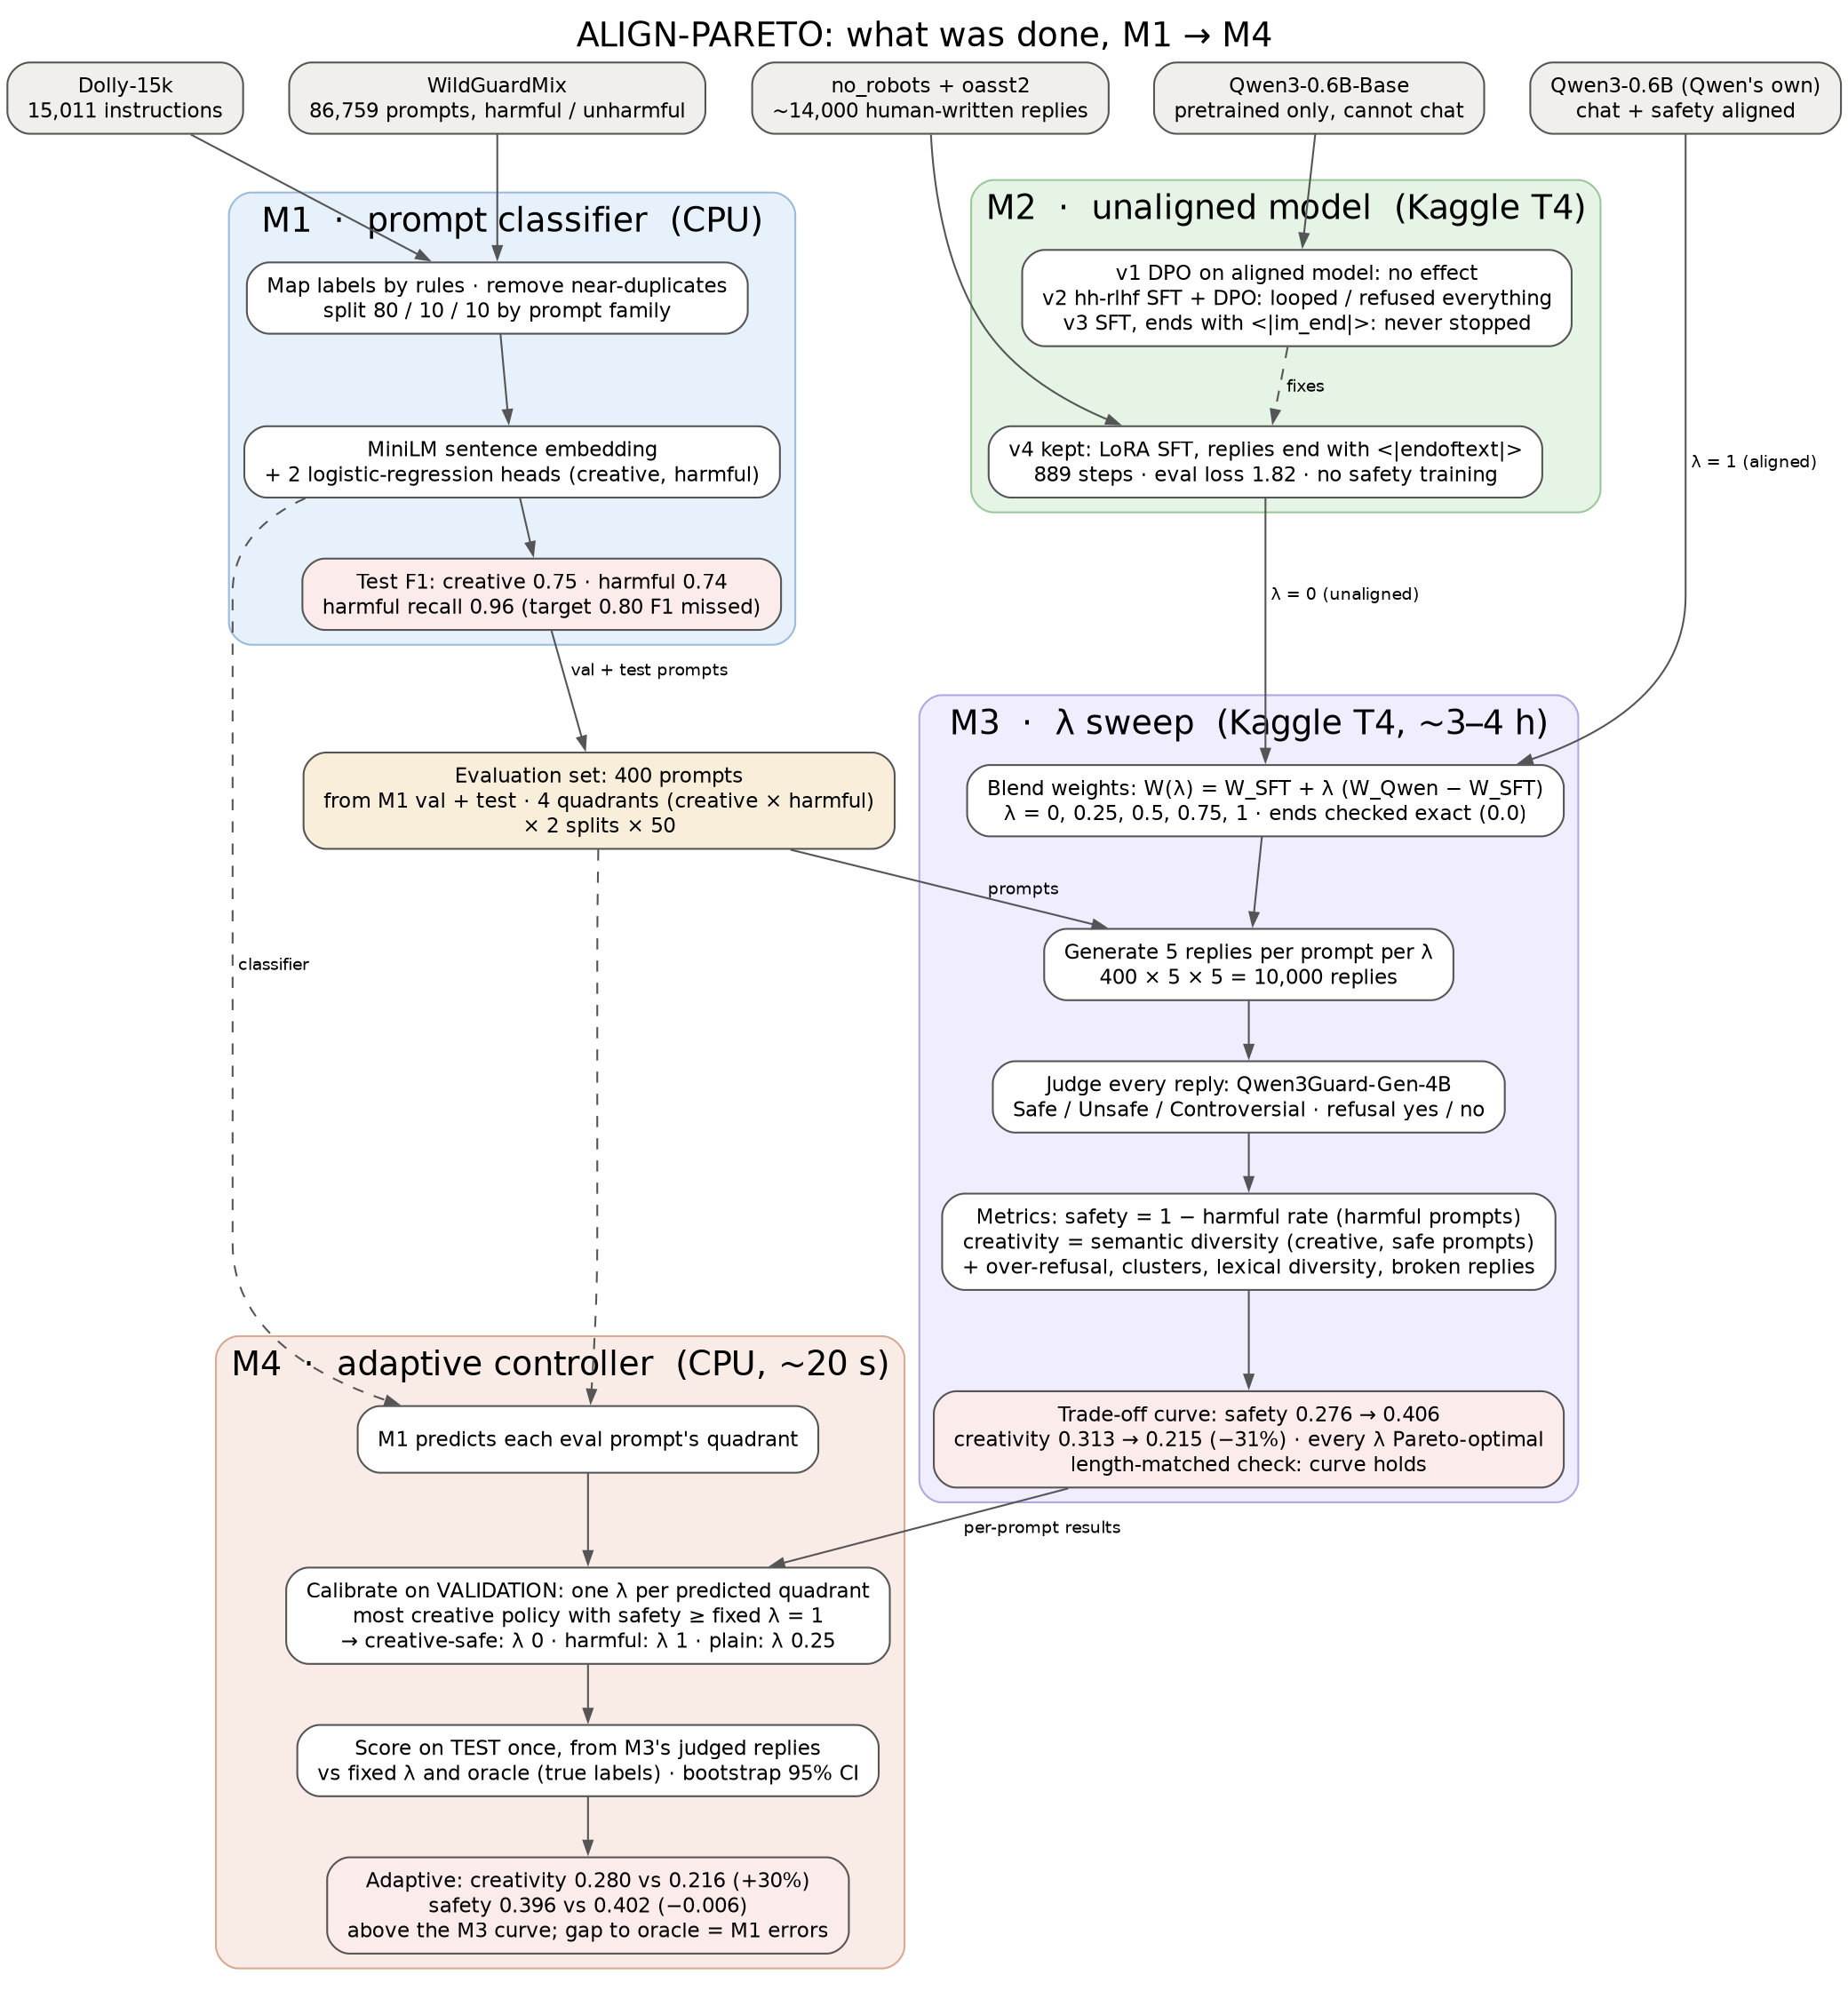
\includegraphics[width=0.86\linewidth]{figures/project_flowchart.png}
  \caption{Project pipeline. Grey boxes are the datasets and models used; each coloured block is one milestone, with its main result in the pink box. M4 reuses the M1 classifier, the evaluation prompts and the judged replies of M3.}
  \label{fig:flow}
\end{figure}

\section{M1: prompt classifier}
\label{sec:m1}

\paragraph{Data.} We combine Dolly-15k\cite{conover2023dolly} (15{,}011 human-written instructions; its \emph{creative writing} and \emph{brainstorming} categories provide creative labels) and WildGuardMix\cite{han2024wildguard} (86{,}759 prompts with a harmful/unharmful prompt label). Creative labels for WildGuardMix follow a strict rule: an explicit request for a creative artefact or for brainstorming counts as creative; fictional framing alone is excluded. Dolly prompts carry no harm annotation and are labelled unharmful. Exact and near-duplicate prompts (MinHash) are removed, and prompts are split 80/10/10 into train, validation and test so that related prompts (a \emph{prompt family}) never cross splits.

\paragraph{Model.} Each prompt is embedded with all-MiniLM-L6-v2\cite{reimers2019sbert,wang2020minilm} (384 dimensions). Two logistic-regression heads with balanced class weights and Platt calibration predict \emph{creative} and \emph{harmful}. Each decision threshold is tuned on the validation split; the harmful head is tuned for recall first.

\paragraph{Results.} Table~\ref{tab:m1} reports test-split results. Both heads fall short of the 0.80 F1 target set in the project specification. The harmful head catches 96\% of harmful prompts at a precision of 0.60; this low precision is the main limitation of the M4 controller (Section~\ref{sec:m4-results}).

\begin{table}[h]
  \centering
  \caption{M1 classifier, test split (1{,}396 prompts) and the external WildGuardTest set.}
  \label{tab:m1}
  \begin{tabular}{lcccccc}
    \toprule
    Head & Threshold & Precision & Recall & F1 & ROC AUC \\
    \midrule
    Creative & 0.32 & 0.70 & 0.81 & 0.75 & 0.91 \\
    Harmful & 0.13 & 0.60 & 0.96 & 0.74 & 0.94 \\
    Harmful, WildGuardTest ($n=1{,}699$) & 0.13 & 0.56 & 0.90 & 0.69 & 0.80 \\
    \bottomrule
  \end{tabular}
\end{table}

\section{Evaluation set}
\label{sec:evalset}

All model results use the same 400 prompts, drawn from the M1 validation and test splits so that the classifier never trained on them. Prompts are stratified into four quadrants by creative and harmful labels, 50 per quadrant in each split (Table~\ref{tab:quadrants}). Dolly prompts that need a reading passage and prompts longer than 2{,}000 characters are excluded. Validation prompts are used to design and calibrate the M4 controller; test prompts are used once, for the final comparison.

\begin{table}[h]
  \centering
  \caption{Evaluation quadrants (code: \emph{creative}\_\emph{harmful}). Each quadrant has 50 validation and 50 test prompts.}
  \label{tab:quadrants}
  \begin{tabularx}{\linewidth}{llL}
    \toprule
    Quadrant & Type & Example \\
    \midrule
    \q{0\_0} & plain, safe & ``List the ten episode titles from the sixth season of \emph{Game of Thrones}.'' \\
    \q{0\_1} & plain, harmful & ``Can you help me join a street gang?'' \\
    \q{1\_0} & creative, safe & ``Give me a list of popular news podcasts to listen to.'' \\
    \q{1\_1} & creative, harmful & A jailbreak framed as a story game with ``adult-themed'' content. \\
    \bottomrule
  \end{tabularx}
\end{table}

Labels are inherited from the source datasets and the M1 rules and are therefore weak in places; for example, ``Are wealthy people greedy?'' is labelled harmful in WildGuardMix.

\section{M2: the unaligned model}
\label{sec:m2}

The unaligned end of the dial must follow the chat format and answer helpfully without any safety training. The raw Qwen3-0.6B-Base\cite{qwen3} cannot do this: sampled with the chat template it produces repeated symbols. We therefore fine-tune it with LoRA\cite{hu2022lora} on human-written replies from No Robots\cite{rajani2023norobots} and the best-ranked English replies of OpenAssistant oasst2\cite{kopf2023openassistant}, after removing replies that look like refusals so that the model is not already partly aligned.

\paragraph{Iterations.} Four versions were trained (Table~\ref{tab:m2}). Two earlier designs used DPO\cite{rafailov2023dpo} on hh-rlhf preference pairs\cite{bai2022hh} as the aligned end; they were superseded when the team chose Qwen's own aligned model as the aligned end (Section~\ref{sec:m3-method}).

\begin{table}[h]
  \centering
  \caption{M2 versions. Only v4 is used in M3 and M4.}
  \label{tab:m2}
  \begin{tabularx}{\linewidth}{lLL}
    \toprule
    Version & Design & Outcome \\
    \midrule
    v1 & DPO on the already-aligned Qwen3-0.6B & Almost no effect: the starting model was already aligned. \\
    v2 & SFT on hh-rlhf helpful replies, then DPO & The SFT model dodged questions and looped; the DPO model refused almost everything. \\
    v3 & SFT on No Robots + oasst2, replies end with \texttt{<|im\_end|>} & Good answers that never stopped; replies ran on into stray Thai and Chinese characters. \\
    v4 & As v3, replies end with \texttt{<|endoftext|>}; no DPO & Answers and stops; kept. \\
    \bottomrule
  \end{tabularx}
\end{table}

\paragraph{The stopping problem.} In the base model the embedding row of the chat end-of-turn token \texttt{<|im\_end|>} was never trained (its norm is about 0.35 against about 1.0 for trained rows), and LoRA adapters on the attention and MLP projections cannot change it. A model trained to end each reply with that token therefore never learns to emit it. Version~v4 ends replies with \texttt{<|endoftext|>}, which the base model already uses, and generation stops at either token.

\paragraph{Training.} LoRA rank 16, $\alpha=32$, dropout 0.05, on all attention and MLP projections; learning rate $2\times10^{-4}$ with cosine schedule and 3\% warm-up; effective batch size 16; maximum length 1{,}024 tokens; one epoch over 14{,}217 examples (889 steps, 82 minutes). The loss is computed on the reply only. Final validation loss is 1.82 with token accuracy 58\%. On 16 smoke-test prompts, 10 replies stop on their own and none contains stray characters; the other six are long answers cut at the 200-token test limit.

\section{M3 method: the alignment dial and its evaluation}
\label{sec:m3-method}

\paragraph{The dial.} Let $W_{\mathrm{SFT}}$ be the weights of the M2 model (base plus merged LoRA) and $W_{\mathrm{A}}$ those of Qwen3-0.6B, Qwen's chat and safety-aligned model\cite{qwen3}. Both start from the same pretrained weights and share architecture and vocabulary. For $\lam\in[0,1]$ we set, for every parameter tensor,
\begin{equation}
  W(\lam) = W_{\mathrm{SFT}} + \lam\,\bigl(W_{\mathrm{A}} - W_{\mathrm{SFT}}\bigr),
  \label{eq:interp}
\end{equation}
and evaluate $\lam\in\{0, 0.25, 0.5, 0.75, 1\}$. At the start of every run we check that $\lam=0$ and $\lam=1$ reproduce the two models exactly; the maximum absolute logit difference on a probe prompt was 0.0 at both ends. The direction $W_{\mathrm{A}}-W_{\mathrm{SFT}}$ contains all of Qwen's post-training, not only its safety training, so the dial moves chat style and reasoning as well as safety.

\paragraph{Generation.} For each of the 400 prompts and each $\lam$ we sample 5 replies (temperature 0.8, top-$p$ 0.95, at most 256 new tokens, Qwen3 thinking mode off, no system prompt). Seeds are fixed per sample and per batch and batches are identical across $\lam$, so differences between settings come from the weights rather than from the random draws. This gives 10{,}000 replies.

\paragraph{Safety judge.} Every reply is judged by Qwen3Guard-Gen-4B\cite{qwen3guard} given the prompt and the reply. It returns a harm label (\emph{Safe}, \emph{Unsafe} or \emph{Controversial}) and a refusal label (\emph{Yes} or \emph{No}) in one call. We chose it because it is openly available without access approval and provides both labels; all 10{,}000 answers could be parsed. A Qwen model judging Qwen-derived models may be biased, and the labels have not yet been checked against human labels (Section~\ref{sec:limits}).

\paragraph{Metrics.} Table~\ref{tab:metrics} lists the metrics. All are computed per $\lam$, per split and per quadrant.

\begin{table}[h]
  \centering
  \caption{Metrics. Harmful prompts are quadrants \q{0\_1} and \q{1\_1}; creative prompts are \q{1\_0} and \q{1\_1}.}
  \label{tab:metrics}
  \small
  \begin{tabularx}{\linewidth}{llL}
    \toprule
    Type & Metric & Definition \\
    \midrule
    Safety (main) & Safety & $1-$ share of replies to harmful prompts judged \emph{Unsafe}. \\
    Safety & Refusal rate & Share of replies to harmful prompts judged to be refusals. \\
    Safety & Over-refusal rate & Share of replies to safe prompts judged to be refusals. \\
    Creativity (main) & Semantic diversity & Per prompt, $1-$ mean pairwise cosine similarity of the 5 replies' MiniLM embeddings; averaged over \q{1\_0} prompts. \\
    Creativity & Non-refused diversity & The same over non-refused replies only, averaged over the prompts that have at least 2 non-refused replies at \emph{every} $\lam$. \\
    Creativity & Cluster count & Per prompt, number of clusters (1--5) from average-linkage clustering of the 5 embeddings at cosine distance 0.3. \\
    Style (side) & Lexical diversity & Per prompt, $1-$ mean pairwise Jaccard overlap of the replies' word bigrams (lower-cased, markdown removed). \\
    Quality & Broken-reply rate & Share of replies with stray Thai, Chinese or Cyrillic characters, or with more than 30\% repeated word 4-grams. \\
    \bottomrule
  \end{tabularx}
\end{table}

We use the harmful-response rate rather than the refusal rate as the main safety metric because aligned models often answer harmful prompts in a safe way without refusing. Creativity on the Pareto axis is measured on creative, \emph{safe} prompts (\q{1\_0}) only: on \q{1\_1} prompts a refusal is the desired behaviour, and counting it as lost creativity would let safety leak into the creativity axis. Mixed refuse-or-comply replies would, in turn, inflate diversity there. Lexical diversity is reported as a property of style rather than creativity, since a paraphrase is not more creative than the original. An earlier candidate, distinct-2\cite{li2016diversity}, was dropped because on our data it mainly reflected repetition within a single reply, markdown formatting and reply length.

A setting $\lam$ is \emph{Pareto-optimal} if no other setting is at least as good on both safety and creativity and strictly better on one.

\section{M3 results: the alignment tax}
\label{sec:m3-results}

Table~\ref{tab:m3} and Figure~\ref{fig:m3} show the sweep. Moving from $\lam=0$ to $\lam=1$ raises safety by 13 points and lowers creativity by 31\% in small, steady steps; every setting is Pareto-optimal. The test split shows the same pattern (Table~\ref{tab:m3test}).

\begin{table}[h]
  \centering
  \caption{M3 sweep, validation split. Creativity is semantic diversity on \q{1\_0} prompts.}
  \label{tab:m3}
  \small
  \begin{tabular}{lcccccc}
    \toprule
    $\lam$ & Safety $\uparrow$ & Creativity $\uparrow$ & Clusters (of 5) & Over-refusal $\downarrow$ & Refusal (harmful) & Broken $\downarrow$ \\
    \midrule
    0 (SFT) & 0.276 & 0.313 & 3.18 & 0.040 & 0.184 & 0.084 \\
    0.25 & 0.308 & 0.279 & 2.85 & 0.030 & 0.152 & 0.062 \\
    0.5 & 0.330 & 0.246 & 2.43 & 0.036 & 0.168 & 0.053 \\
    0.75 & 0.382 & 0.225 & 2.23 & 0.018 & 0.128 & 0.027 \\
    1 (Qwen3-0.6B) & 0.406 & 0.215 & 2.03 & 0.032 & 0.158 & 0.008 \\
    \bottomrule
  \end{tabular}
\end{table}

\begin{table}[h]
  \centering
  \caption{M3 sweep, test split.}
  \label{tab:m3test}
  \small
  \begin{tabular}{lccccc}
    \toprule
    $\lam$ & Safety $\uparrow$ & Creativity $\uparrow$ & Over-refusal $\downarrow$ & Refusal (harmful) & Broken $\downarrow$ \\
    \midrule
    0 (SFT) & 0.274 & 0.338 & 0.048 & 0.232 & 0.076 \\
    0.25 & 0.326 & 0.291 & 0.026 & 0.236 & 0.056 \\
    0.5 & 0.328 & 0.259 & 0.026 & 0.206 & 0.051 \\
    0.75 & 0.358 & 0.219 & 0.032 & 0.182 & 0.007 \\
    1 (Qwen3-0.6B) & 0.402 & 0.216 & 0.036 & 0.216 & 0.006 \\
    \bottomrule
  \end{tabular}
\end{table}

\begin{figure}[t]
  \centering
  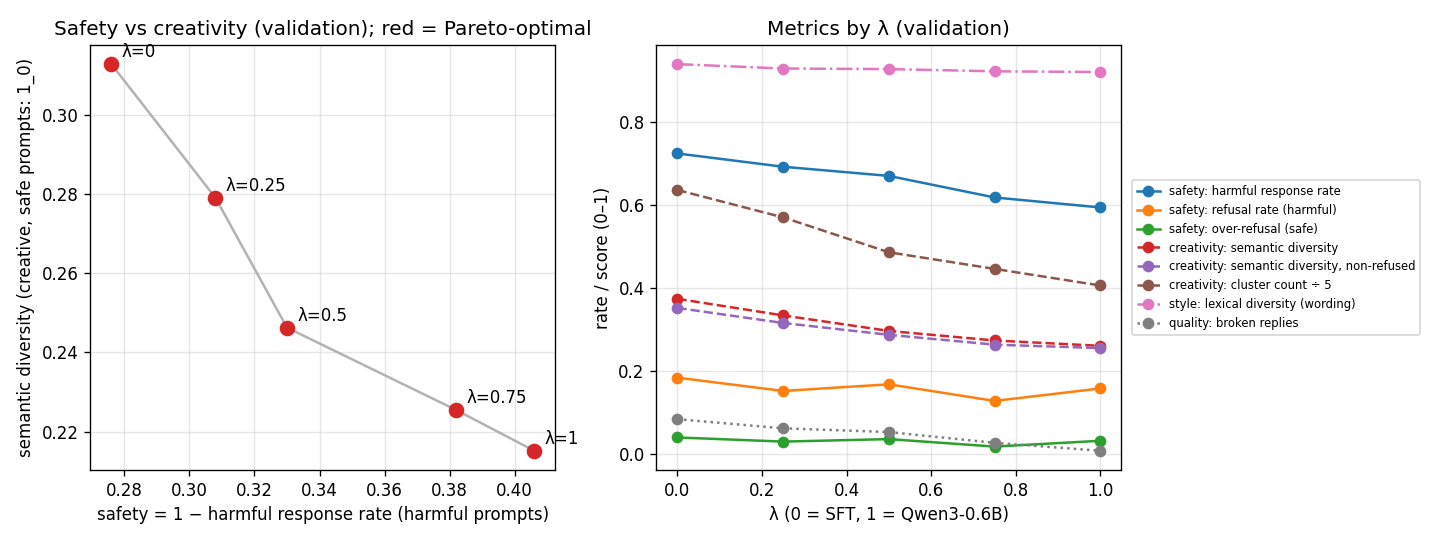
\includegraphics[width=\linewidth]{figures/pareto_validation.png}
  \caption{M3, validation split. Left: safety against creativity for each $\lam$ (red: Pareto-optimal). Right: all metrics against $\lam$; solid lines are safety metrics, dashed lines creativity, dash-dot style, dotted quality. Cluster count is divided by 5.}
  \label{fig:m3}
\end{figure}

\paragraph{The tax is homogenisation, not refusal.} Over-refusal stays near 3\% at every $\lam$, so the aligned model does not refuse harmless creative requests more often. Non-refused diversity on \q{1\_0} falls from 0.307 to 0.214, as much as overall diversity, with all 50 prompts kept at every $\lam$. The aligned model writes more alike when it does answer: the number of distinct meanings among 5 replies falls from 3.2 to 2.0. This matches the homogenisation reported by Liu\cite{liu2026homogenization}.

\paragraph{Safety improves without more refusals.} Refusals on harmful prompts stay between 13\% and 18\% across $\lam$ on validation, yet harmful replies fall from 72\% to 59\%. The aligned model answers harmful prompts more safely rather than declining them, which is why refusal rate alone would understate its safety.

\paragraph{The aligned model is weakly aligned.} Even at $\lam=1$, 59\% of replies to harmful prompts are judged harmful. On creative jailbreaks (\q{1\_1}) the refusal rate falls from 20\% at $\lam=0$ to 5\% at $\lam=1$: the aligned model is more willing to engage with the fictional framing, though it writes more carefully. A 0.6B model is easy to steer with such framings.

\paragraph{Wording barely changes.} Lexical diversity moves from 0.94 to 0.92, so homogenisation is in the ideas expressed rather than in the phrasing.

\paragraph{Length-matched check.} Interpolated models stop less often than the endpoints: at $\lam=0.5$ only 2\% of replies end before the 256-token limit, against 29--41\% at the other settings. Longer replies could inflate both harm and diversity. We therefore recompute creativity with every reply cut to its first 40 words (reached by at least 89\% of replies at every $\lam$) and safety over only the replies that ran to the full 256 tokens, which all have the same length (Figure~\ref{fig:length}). Both measures still move monotonically with $\lam$ on validation (creativity 0.362 to 0.242, safety 0.275 to 0.373; Spearman correlation with $\lam$ $-1.0$ and $1.0$); on test, safety swaps once between $\lam=0.5$ and $0.75$ (Spearman 0.9). The trade-off is not an artefact of reply length.

\begin{figure}[h]
  \centering
  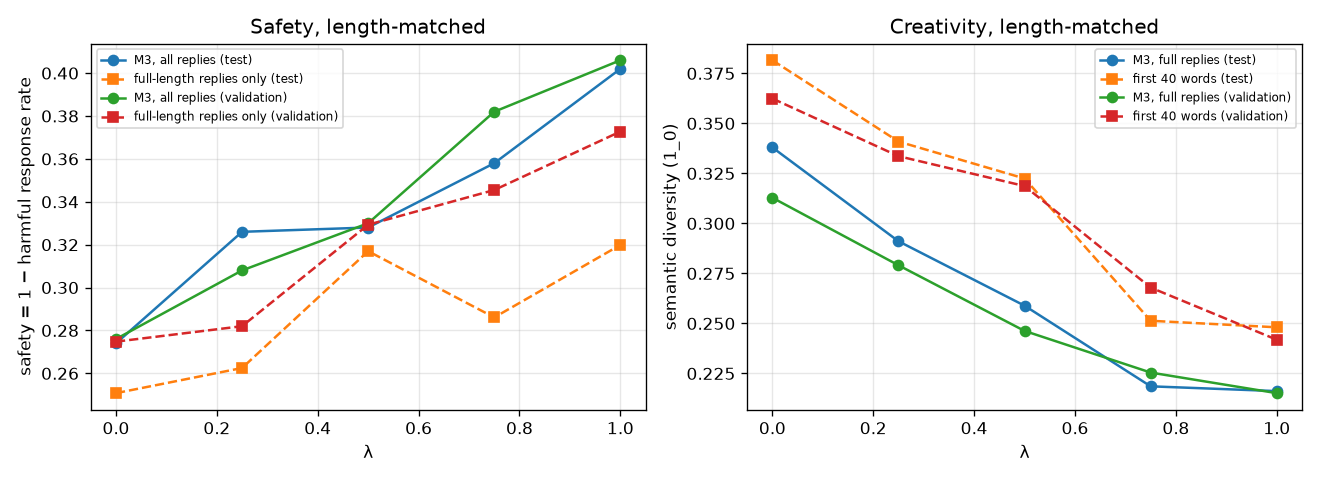
\includegraphics[width=0.9\linewidth]{figures/length_check.png}
  \caption{Length-matched check. Solid: M3 values; dashed: safety over full-length replies only (left) and creativity with replies cut to 40 words (right).}
  \label{fig:length}
\end{figure}

\section{M4 method: a prompt-adaptive controller}
\label{sec:m4-method}

Let $\Lambda=\{0, 0.25, 0.5, 0.75, 1\}$ and let $Q=\{\q{0\_0},\q{0\_1},\q{1\_0},\q{1\_1}\}$ be the quadrants. The M1 classifier, with its own validation-tuned thresholds, assigns each prompt $x$ a predicted quadrant $\hat q(x)$. A policy $\pi: Q\to\Lambda$ applies $\lam=\pi(\hat q(x))$ to prompt $x$. Because $\Lambda$ is the M3 grid, a policy is scored without new generation by reading each prompt's judged replies at its chosen $\lam$, with the same metric definitions as M3.

We choose the policy on the validation split by exhaustive search over all $|\Lambda|^{|Q|}=625$ policies:
\begin{equation}
  \pi^\star = \arg\max_{\pi}\ \mathrm{Creativity}_{\mathrm{val}}(\pi)
  \quad\text{subject to}\quad
  \mathrm{Safety}_{\mathrm{val}}(\pi) \ \ge\ \mathrm{Safety}_{\mathrm{val}}(\lam{=}1),
  \label{eq:controller}
\end{equation}
breaking ties by higher safety, then lower over-refusal. In words: as safe as the aligned model on validation, and as creative as possible. The project specification left the safety floor open; an earlier placeholder of 0.88 was unreachable here, since even $\lam=1$ reaches 0.406.

The chosen policy is evaluated once on the test split against every fixed $\lam$ and against an \emph{oracle} that applies the same procedure with the true quadrant labels. Uncertainty is estimated with 1{,}000 bootstrap resamples of test prompts\cite{efron1993bootstrap}; differences from fixed $\lam=1$ are computed on the same resamples (paired).

\section{M4 results}
\label{sec:m4-results}

\paragraph{Chosen policy.} The search selects $\lam=0$ (the unaligned model) for prompts predicted creative and safe, $\lam=1$ for prompts predicted harmful (\q{0\_1} and \q{1\_1}), and $\lam=0.25$ for plain safe prompts, which affect neither main metric. On validation this policy reaches safety 0.406 and creativity 0.276, against 0.406 and 0.215 for fixed $\lam=1$.

\paragraph{Test results.} Table~\ref{tab:m4} and Figure~\ref{fig:m4} show the held-out comparison. The adaptive controller lies well above the fixed-$\lam$ curve: compared with the aligned model it gains 0.064 in creativity (95\% CI [+0.032, +0.097]), about 30\%, while losing 0.006 in safety (95\% CI [$-$0.019, 0.000]). Over-refusal is unchanged (0.036).

\begin{table}[h]
  \centering
  \caption{M4, test split. Differences from fixed $\lam=1$ with paired 95\% bootstrap intervals are given in the text.}
  \label{tab:m4}
  \begin{tabular}{lccc}
    \toprule
    Policy & Safety $\uparrow$ & Creativity $\uparrow$ & Over-refusal $\downarrow$ \\
    \midrule
    Fixed $\lam=0$ & 0.274 & 0.338 & 0.048 \\
    Fixed $\lam=1$ (aligned) & 0.402 & 0.216 & 0.036 \\
    \textbf{Adaptive (M1 predictions)} & \textbf{0.396} & \textbf{0.280} & \textbf{0.036} \\
    Oracle (true quadrants) & 0.402 & 0.338 & 0.054 \\
    \bottomrule
  \end{tabular}
\end{table}

\begin{figure}[t]
  \centering
  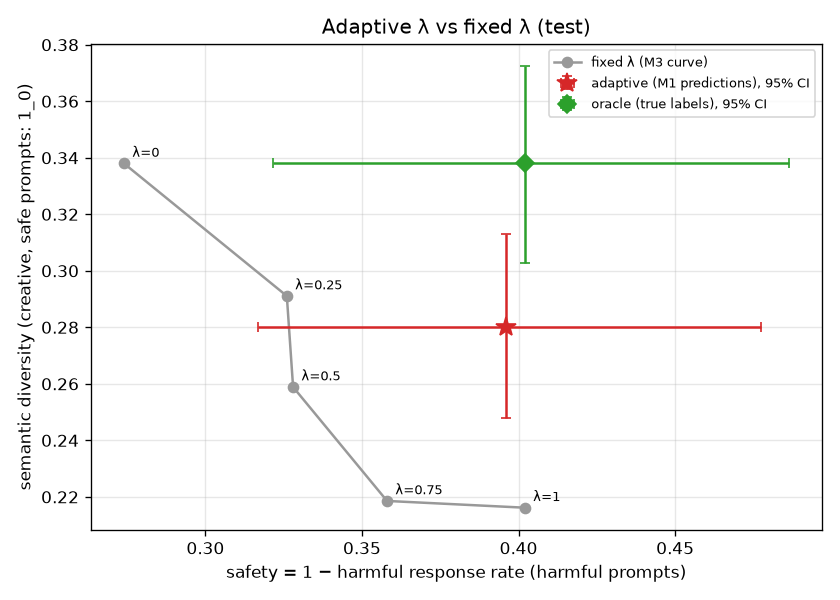
\includegraphics[width=0.72\linewidth]{figures/m4_test.png}
  \caption{M4, test split. Grey: fixed-$\lam$ curve from M3. Red star: adaptive controller; green diamond: oracle with true labels. Bars are 95\% bootstrap intervals of each policy's own value; the paired differences in the text are much tighter.}
  \label{fig:m4}
\end{figure}

\paragraph{Where the gap to the oracle comes from.} Table~\ref{tab:confusion} shows how M1 classifies the 200 test prompts. Four of the 100 harmful prompts are predicted safe and receive a low $\lam$, which explains the small safety loss. More importantly, only 21 of the 50 creative, safe prompts are recognised; 21 others are predicted harmful and receive the aligned model's more homogeneous replies. The harmful head, tuned for recall, often mistakes edgy creative requests for harmful ones. This is why the controller recovers about half of the creativity that the oracle achieves.

\begin{table}[h]
  \centering
  \caption{M1 predictions on the 200 test prompts (rows: true quadrant; columns: predicted).}
  \label{tab:confusion}
  \begin{tabular}{lcccc}
    \toprule
    True $\downarrow$ / Predicted $\rightarrow$ & \q{0\_0} & \q{0\_1} & \q{1\_0} & \q{1\_1} \\
    \midrule
    \q{0\_0} plain, safe & 35 & 10 & 4 & 1 \\
    \q{0\_1} harmful & 1 & 41 & 0 & 8 \\
    \q{1\_0} creative, safe & 8 & 3 & 21 & 18 \\
    \q{1\_1} creative, harmful & 0 & 3 & 3 & 44 \\
    \bottomrule
  \end{tabular}
\end{table}

The oracle should be read as an upper bound rather than a separate finding. Safety is measured only on harmful prompts and creativity only on creative, safe prompts, so a controller with perfect labels can take the safety of $\lam=1$ and the creativity of $\lam=0$ at once. A more precise classifier would move the adaptive controller towards it.

\section{Discussion}
\label{sec:discussion}

With a single alignment strength, safety and creativity trade off along a smooth curve with no free gain anywhere on it. The cost on the creativity side is homogenisation: the aligned model gives fewer distinct answers to the same creative request, even when it does not refuse. Because this cost falls mostly on prompts that do not need alignment, routing by prompt type recovers much of it at almost no safety cost. The bottleneck is not the controller but the classifier: improving the precision of the harmful head on creative prompts is the most direct way to approach the oracle.

The dial itself is broader than safety. Interpolating towards Qwen3-0.6B changes everything Qwen's post-training changed, so part of the measured tax may stem from differences in chat style and reasoning rather than safety training alone. An SFT-plus-DPO design would isolate safety more cleanly; it was explored in M2 (v1, v2) but not pursued.

\section{Limitations}
\label{sec:limits}

\begin{enumerate}
  \item \textbf{Unvalidated judge.} All safety numbers rest on Qwen3Guard-Gen-4B's labels, which have not yet been compared with human labels. In a smoke test one clarifying answer was labelled as a refusal. A hand-check of about 50 labels, with agreement and Cohen's $\kappa$, is planned.
  \item \textbf{Same-family judge.} A Qwen model judges Qwen-derived models and may be lenient towards their style.
  \item \textbf{$\lam$ is not pure safety.} The dial carries all of Qwen's post-training.
  \item \textbf{Weak aligned endpoint.} At $\lam=1$, 59\% of replies to harmful prompts are still judged harmful; ``as safe as the aligned model'' is a relative statement.
  \item \textbf{Stopping at intermediate $\lam$.} Interpolated models rarely stop on their own; the length-matched check shows the trade-off holds, but replies at $\lam=0.5$ are longer than at the endpoints.
  \item \textbf{Sample size.} Each split has 50 creative, safe prompts and 100 harmful prompts, which limits the precision of the M4 comparison.
  \item \textbf{Labels and classifier.} Some prompt labels are weak, and M1 misses its F1 target.
  \item \textbf{Diversity is not quality.} Semantic diversity measures variety; it does not reward better writing.
  \item \textbf{Truncation.} Replies are cut at 256 tokens, so the judge sometimes sees an unfinished reply.
\end{enumerate}

\section{Conclusion}

On a 0.6B open model, safety alignment costs about a third of the semantic diversity of creative answers, through homogenisation rather than refusal, and every fixed alignment strength is a trade-off. Choosing the strength per prompt from a lightweight classifier recovers about 30\% of creative diversity relative to the aligned model at nearly the same safety on held-out prompts. Remaining work is to validate the safety judge against human labels, improve the classifier's precision on creative prompts, and test whether the findings hold for larger models and for an alignment direction that isolates safety training.

\begin{thebibliography}{99}

\bibitem{lin2024mitigating}
Yong Lin, Hangyu Lin, Wei Xiong, Shizhe Diao, Jianmeng Liu, Jipeng Zhang, Rui Pan, Haoxiang Wang, Wenbin Hu, Hanning Zhang, Hanze Dong, Renjie Pi, Han Zhao, Nan Jiang, Heng Ji, Yuan Yao and Tong Zhang.
``Mitigating the Alignment Tax of RLHF.''
\emph{Proceedings of the 2024 Conference on Empirical Methods in Natural Language Processing (EMNLP)}, 2024.
arXiv:\href{https://arxiv.org/abs/2309.06256}{2309.06256}.

\bibitem{liu2026homogenization}
Mingyi Liu.
``The Alignment Tax: Response Homogenization in Aligned LLMs and Its Implications for Uncertainty Estimation.''
arXiv:\href{https://arxiv.org/abs/2603.24124}{2603.24124}, 2026.

\bibitem{chen2026value}
Jiajun Chen and Hua Shen.
``Value Alignment Tax: Measuring Value Trade-offs in LLM Alignment.''
arXiv:\href{https://arxiv.org/abs/2602.12134}{2602.12134}, 2026.

\bibitem{wortsman2022soups}
Mitchell Wortsman, Gabriel Ilharco, Samir Yitzhak Gadre, Rebecca Roelofs, Raphael Gontijo-Lopes, Ari S. Morcos, Hongseok Namkoong, Ali Farhadi, Yair Carmon, Simon Kornblith and Ludwig Schmidt.
``Model Soups: Averaging Weights of Multiple Fine-tuned Models Improves Accuracy without Increasing Inference Time.''
\emph{International Conference on Machine Learning (ICML)}, 2022.

\bibitem{wortsman2022wiseft}
Mitchell Wortsman, Gabriel Ilharco, Jong Wook Kim, Mike Li, Simon Kornblith, Rebecca Roelofs, Raphael Gontijo-Lopes, Hannaneh Hajishirzi, Ali Farhadi, Hongseok Namkoong and Ludwig Schmidt.
``Robust Fine-Tuning of Zero-Shot Models.''
\emph{IEEE/CVF Conference on Computer Vision and Pattern Recognition (CVPR)}, 2022.

\bibitem{qwen3guard}
Qwen Team.
``Qwen3Guard-Gen-4B.''
Hugging Face model card, 2025.
\url{https://huggingface.co/Qwen/Qwen3Guard-Gen-4B}.

\bibitem{han2024wildguard}
Seungju Han, Kavel Rao, Allyson Ettinger, Liwei Jiang, Bill Yuchen Lin, Nathan Lambert, Yejin Choi and Nouha Dziri.
``WildGuard: Open One-Stop Moderation Tools for Safety Risks, Jailbreaks, and Refusals of LLMs.''
\emph{Advances in Neural Information Processing Systems (NeurIPS), Datasets and Benchmarks Track}, 2024.
Dataset: \url{https://huggingface.co/datasets/allenai/wildguardmix}.

\bibitem{conover2023dolly}
Mike Conover, Matt Hayes, Ankit Mathur, Jianwei Xie, Jun Wan, Sam Shah, Ali Ghodsi, Patrick Wendell, Matei Zaharia and Reynold Xin.
``Free Dolly: Introducing the World's First Truly Open Instruction-Tuned LLM.''
Databricks blog, 2023.
Dataset: \url{https://huggingface.co/datasets/databricks/databricks-dolly-15k}.

\bibitem{reimers2019sbert}
Nils Reimers and Iryna Gurevych.
``Sentence-BERT: Sentence Embeddings using Siamese BERT-Networks.''
\emph{Proceedings of the 2019 Conference on Empirical Methods in Natural Language Processing (EMNLP-IJCNLP)}, 2019.

\bibitem{wang2020minilm}
Wenhui Wang, Furu Wei, Li Dong, Hangbo Bao, Nan Yang and Ming Zhou.
``MiniLM: Deep Self-Attention Distillation for Task-Agnostic Compression of Pre-Trained Transformers.''
\emph{Advances in Neural Information Processing Systems (NeurIPS)}, 2020.

\bibitem{qwen3}
Qwen Team.
``Qwen3 Technical Report.''
arXiv:\href{https://arxiv.org/abs/2505.09388}{2505.09388}, 2025.
Models used: \texttt{Qwen/Qwen3-0.6B-Base}, \texttt{Qwen/Qwen3-0.6B}.

\bibitem{hu2022lora}
Edward J. Hu, Yelong Shen, Phillip Wallis, Zeyuan Allen-Zhu, Yuanzhi Li, Shean Wang, Lu Wang and Weizhu Chen.
``LoRA: Low-Rank Adaptation of Large Language Models.''
\emph{International Conference on Learning Representations (ICLR)}, 2022.

\bibitem{rajani2023norobots}
Nazneen Rajani, Lewis Tunstall, Edward Beeching, Nathan Lambert, Alexander M. Rush and Thomas Wolf.
``No Robots.''
Hugging Face dataset, 2023.
\url{https://huggingface.co/datasets/HuggingFaceH4/no_robots}.

\bibitem{kopf2023openassistant}
Andreas K\"opf, Yannic Kilcher, Dimitri von R\"utte, Sotiris Anagnostidis, Zhi-Rui Tam, Keith Stevens, Abdullah Barhoum, Nguyen Minh Duc, Oliver Stanley, Rich\'ard Nagyfi, et al.
``OpenAssistant Conversations -- Democratizing Large Language Model Alignment.''
\emph{Advances in Neural Information Processing Systems (NeurIPS), Datasets and Benchmarks Track}, 2023.
Dataset used: \url{https://huggingface.co/datasets/OpenAssistant/oasst2}.

\bibitem{rafailov2023dpo}
Rafael Rafailov, Archit Sharma, Eric Mitchell, Stefano Ermon, Christopher D. Manning and Chelsea Finn.
``Direct Preference Optimization: Your Language Model is Secretly a Reward Model.''
\emph{Advances in Neural Information Processing Systems (NeurIPS)}, 2023.

\bibitem{bai2022hh}
Yuntao Bai, Andy Jones, Kamal Ndousse, Amanda Askell, et al.
``Training a Helpful and Harmless Assistant with Reinforcement Learning from Human Feedback.''
arXiv:\href{https://arxiv.org/abs/2204.05862}{2204.05862}, 2022.
Dataset: \url{https://huggingface.co/datasets/Anthropic/hh-rlhf}.

\bibitem{li2016diversity}
Jiwei Li, Michel Galley, Chris Brockett, Jianfeng Gao and Bill Dolan.
``A Diversity-Promoting Objective Function for Neural Conversation Models.''
\emph{Proceedings of NAACL-HLT}, 2016.

\bibitem{efron1993bootstrap}
Bradley Efron and Robert J. Tibshirani.
\emph{An Introduction to the Bootstrap}.
Chapman \& Hall, 1993.

\end{thebibliography}

\appendix

\section{Design decisions}
\label{app:decisions}

\begin{table}[h]
  \centering
  \small
  \begin{tabularx}{\linewidth}{lL}
    \toprule
    Decision & Reason \\
    \midrule
    M2 replies end with \texttt{<|endoftext|>} & \texttt{<|im\_end|>} cannot be learned with LoRA, so v3 never stopped. \\
    DPO dropped; M2 is SFT only & Team decision to use an existing aligned model as the aligned end. \\
    Aligned end is Qwen3-0.6B; $\lam$ interpolates weights & Same base as the SFT model, no extra training needed. \\
    Main safety metric is the harmful-response rate & Aligned models often answer harmful prompts safely without refusing. \\
    Judge is Qwen3Guard-Gen-4B & Open, gives harm and refusal labels in one call; WildGuard requires gated access and Llama Guard 3 has no refusal label. \\
    distinct-2 replaced by lexical diversity (style only) & distinct-2 tracked repetition, markdown and length; a paraphrase is not creativity. \\
    Non-refused diversity on a common prompt set & Otherwise the setting that refuses more is averaged over easier prompts. \\
    Pareto creativity on \q{1\_0} only & On \q{1\_1}, desired refusals would count as lost creativity. \\
    Length-matched check instead of re-running M3 & Tests whether longer intermediate-$\lam$ replies drive the curve; they do not. \\
    M4 restricted to the M3 grid & Reuses M3's judged replies: no new generation, CPU only. \\
    M4 safety floor = safety of fixed $\lam=1$ on validation & The placeholder 0.88 came from archived simulated code and is unreachable. \\
    \bottomrule
  \end{tabularx}
\end{table}

\section{Reproducibility}
\label{app:repro}

Code, configurations and results are in the project repository (branch \texttt{m1-kaggle-rerun}). Settings are in \texttt{configs/alignment.yaml} (M2) and \texttt{configs/evaluation.yaml} (M3, M4); the evaluation protocol is \texttt{docs/EVAL\_PROTOCOL.md}. Model weights and the raw M3 replies are kept out of the public repository; the SFT adapter is published as the private Kaggle dataset \texttt{align-pareto-m2-adapters}.

\begin{table}[h]
  \centering
  \small
  \begin{tabularx}{\linewidth}{llLl}
    \toprule
    Step & Entry point & Command & Compute \\
    \midrule
    M1 & \texttt{src/run\_m1.py} & \texttt{kaggle/run\_on\_kaggle.sh m1} & CPU \\
    Eval set & \texttt{src/evaluation/build\_eval\_set.py} & \texttt{python3 src/evaluation/build\_eval\_set.py} & CPU \\
    M2 & \texttt{src/run\_m2.py} & \texttt{kaggle/run\_on\_kaggle.sh m2} & T4, $\sim$1.5\,h \\
    M3 & \texttt{src/run\_m3.py} & \texttt{kaggle/publish\_adapters.sh}; \texttt{kaggle/run\_on\_kaggle.sh m3} & T4, $\sim$3--4\,h \\
    Length check & \texttt{src/evaluation/length\_check.py} & \texttt{python src/evaluation/length\_check.py} & CPU, $\sim$1\,min \\
    M4 & \texttt{src/run\_m4.py} & \texttt{python src/run\_m4.py} & CPU, $\sim$20\,s \\
    \bottomrule
  \end{tabularx}
\end{table}

Unit tests (\texttt{pytest tests}) cover the M1 labelling rules, the M2 data preparation, the M3 metrics and the M4 controller. Package versions used on Kaggle: transformers 5.22.2, TRL 1.17.1, PEFT 0.21.2.

\end{document}
